\documentclass[output=paper]{LSP/langsci}  
\author{P. Stoeckle\affiliation{University of Zürich}} 
\title{Horizontal and vertical variation in Swiss German morphosyntax}
\abstract{This paper deals with the question of how areas with different syntactic variability can be identified. It uses data from the ‘Syntactic Atlas of German-speaking Switzerland‘ (SADS) which uses multiple informants in each survey location. As a starting point the well-known doubling construction with the verb \emph{aafange} ‘begin’ is used to illustrate how the different regions differ with respect to inter-personal variation and how the different variants can be mapped in terms of predominance, i.e. to what extent they co-occur or compete with the other variants. As a quantitative measure, the intensity value of the dominant variant (i.e. the agreement rate between those informants providing the dominant variant as their variant) is used as the basis to create a so-called “variation index”. This technique is applied to a larger set of SADS data, and the results are mapped onto the survey points indicating the syntactic variability for each location. To assess the validity of the method, several subgroups are created which turn out to correlate with the whole data set at a significant level. By performing a hot spot analysis, regional clusters of high/low syntactic variability can be identified. 
}

\maketitle 
\begin{document}
 
   

\section{Introduction}
In traditional dialectological surveys, linguistic variation has been viewed as one-dimensional, i.e. the only level of interest has been the geographical level. The main focus of most atlas projects\footnote{ An exception would be the \emph{Mittelrheinischer Sprachatlas} (\emph{MRhSA}; ‘Linguistic Atlas of the Middle Rhine’; \citealt{bellmann_mittelrheinischer_1994}), for which informants with different social backgrounds were taken into account.} was documentation, since researchers aimed at investigating the old base dialects. Therefore, only one speaker – who was assumed to represent the dialect in its most original form – was interviewed at each location. While these atlases generally provide a very profound and extensive overview of the traditional linguistic structurings of the areas under investigation, sociolinguistic findings as well as everyday experience suggest that the equation \emph{one place} = \emph{one variety} does not correspond to linguistic reality, rather we find inter- and even intra-speaker variation at single locations.

A second observation regarding traditional dialect atlases is that (morpho-)syntax has often been largely excluded from surveys. As for the \emph{Sprachatlas der deutschen Schweiz} (\emph{SDS}; ‘Linguistic Atlas of German-speaking Switzerland’, \cite{hotzenkocherle_sprachatlas_1962}), only seven maps (0.8\%; \citealt[42]{bucheli_syntactic_2002}) depict syntactic phenomena. The main objections raised by traditional dialectologists were that syntactic phenomena of dialects do not show any geographical distribution and that dialect syntax basically is the syntax of spoken language and thus does not display many differences to the spoken standard language \citep[109]{loffler_dialektologie._2003}.

However, in recent years a growing interest in the study of dialect syntax can be observed, initiated by theoretical linguists who discovered dialects as an ideal empirical basis for the study of microvariation \citep{kayne_microparametric_1996}. As a result, a number of projects in many different countries were initialized.\footnote{ The Edisyn (\emph{European Dialect Syntax}) website gives an overview of recent projects on dialect syntax (\url{http://www.dialectsyntax.org/wiki/Welcome} [accessed November 2014]).} One of these projects is the \emph{Syntaktischer Atlas der deutschen Schweiz} (\emph{SADS}; ‘Syntactic Atlas of German-speaking Switzerland’; \citealt{bucheli_syntactic_2002}) which provides the data for my analyses in this paper. In contrast to many of the aforementioned traditional atlas projects, in the SADS survey multiple informants were investigated at each location. This gives us the opportunity to analyze syntactic variation not only on one dimension, i.e. on the horizontal level (\emph{between} locations), but to include the vertical level (\emph{between} informants \emph{at} single locations) as a second dimension.\footnote{It should be noted that my approach resembles, to a certain degree, the concept of “two-dimensionality” taken in the MRhSA \citep{bellmann_zur_1997}. While the selection of speakers was more systematic in the MRhSA since informants from two groups of clearly defined social backgrounds were interviewed, in my analysis I deal with multiple informants at each location. This means that for now inter-speaker variation is examined regardless of the informants’ social backgrounds.} 

From a theoretical perspective, the concept of variation is important in (at least) two respects: On the one hand, it is seen in a close relationship with language change and is often regarded as an indicator thereof. However, it is not clear whether variation is to be seen as a precondition for language change or as its consequence \citep[39--40]{glaser_wandel_2014} --- or if both cases are possible, depending on the linguistic phenomenon and the extra-linguistic context. On the other hand (and closely connected to the first aspect), in recent years there have been more and more attempts to integrate the concept of variation into syntactic theory \citep{cornips_syntax_2005}. The central question guiding this approach is whether variation or optionality can be assumed an inherent part of grammar \citep{seiler_syntaxgeographie_2008} or have to be generally excluded, in which case variation would be the result of (different) competing grammars (\citealt{kroch_morphosyntactic_1994}; cf. Henry 2002 %MISSING REF 
for a general discussion of that matter). While in the first case variation could be seen as “Normalzustand” (‘normal state’; \citealt[56]{seiler_syntaxgeographie_2008}), thus providing a basis for language change, in the latter case variation would be a reflex of change “proceed[ing] via competition between grammatically incompatible options which substitute for one another in usage” \citep[180]{kroch_morphosyntactic_1994}.

The goal of this paper is to take a closer look at interpersonal variation and to classify the whole research area into regions according to this variation. For this purpose, a variation index will be developed. While the focus of this paper is on the methodology, the measure of variation will nevertheless provide a useful tool for dealing with the theoretical issues described above, and it will help us answer the following questions: Which regions show the most variation and which regions show only little variation? Can a high degree of variability be regarded as an indicator for \emph{dynamism} or \emph{modernism}, and does little variation indicate a linguistically \emph{static} or \emph{conservative} situation? How do the resulting geographic patterns correlate with other findings from Swiss-German dialectology? The answers to these questions shall help us gain a better understanding of speech variation, linguistic change and the relationship between them.

\section{An example from the Syntactic Atlas of German-speaking Switzerland (\emph{SADS})}

Before I illustrate the syntactic variability on the basis of one phenomenon, I will provide a quick overview of the database. The SADS project was funded by the Swiss National Science Foundation between the years 2000 and 2008 and was extended through the end of 2014. The survey was conducted using four written questionnaires including 118 questions on 54 different syntactic variables. These questionnaires were sent to informants in 383 locations which were chosen as a subset of the 600 places included in the SDS survey. The goal was to include ten informants at each location: men and women, different age groups and all kinds of professions \citep[52]{bucheli_syntactic_2002}. Apart from the general requirement of localness, the informants were not acquired systematically, so their numbers as well as their socio-demographic backgrounds are not evenly distributed over the research area. Finally, a total of 3187 informants (i.e. an average of 8 informants per location) could be included in the survey. Since not all of them were able to complete all four questionnaires (due to lack of time, migration, illness or death), a total of 2770 informants answered the whole series of questionnaires \citep[33]{berger_neue_2008}. For the elicitation of the data, different question types were used: \emph{translation} from the standard language into the informants’ dialect, \emph{completion} with a dialectal beginning of a sentence which was to be completed, and \emph{multiple choice} with several given answers from among which the participants could indicate which ones they would accept and which they would prefer.\footnote{For more information cf. the project website: \url{http://www.ds.uzh.ch/dialektsyntax/} [accessed November 2014].}

The following example refers to the syntax of the verb \emph{anfangen} (‘to begin’). In Swiss German, the verb \emph{anfangen} (or, in its dialectal form, \emph{aafaa}) belongs to a group of verbs which allow for (or, in some areas, require) a repetition of a reduced form of the verb when governing an infinitive.\footnote{The other verbs are \emph{gehen} (‘to go’), \emph{kommen} (‘to come’) and \emph{lassen} (‘to let’). For more information on the phenomenon cf. \citet{glaser_empirische_2011} and \citet{lotscher_zur_1993}.} In the SADS questionnaires, six items addressed the syntax of the verb \emph{anfangen}. Example (1) illustrates the replacement of the particle \emph{an} by the reduced infinitival form \textsc{afa}.

\ea %1
\label{ex:1}
%\langinfo{lg}{fam}{src}\\
\gll [dann]  fängt  das Eis  \textsc{afa} schmelzen.\\
[then]    begins  the ice    \textsc{begin}  melt.	\\
\glt `Then the ice begins to melt.'
\z

The main interest in the SADS survey regarding this phenomenon was to investigate in which regions the doubling of \textsc{afa}\footnote{ This is a rather simplified description of the phenomenon as it could be argued that it is rather the element \emph{{}-fa} which is doubled than the whole form \textsc{afa}. For more details about the occurrence of \textsc{afa} in different syntactic contexts cf. \citet{andres_verdoppelung_2011}.} would occur and whether it was exclusive or optional. The respective task for the informants was to translate the following sentence into their own dialect (this was the first question of the third questionnaire):
\vskip11pt
\emph{Wenn es so warm bleibt, fängt das Eis an zu schmelzen!} (‘If it stays this warm, the ice will begin to melt’)
\vskip11pt
Altogether 2835 answers given by 2761 informants could be used,\footnote{In very few cases the answers could not be included since the informants had not understood the purpose of the questionnaire properly.} among which the most frequent were the following:

\begin{enumerate}
\item \emph{… fängt das Eis an (zu) schmelzen} (begins the ice \textsc{part} (to) melt; ‘the ice begins to melt’; 1417 answers)\footnote{ Only 138 of these translations were realized with the infinitival particle \emph{zu}, 1279 were realized without it.}

\item \emph{… fängt das Eis }\emph{\textsc{afa}}\emph{ schmelzen} (begins the ice \textsc{begin} melt; 959 answers)

\item \emph{… schmilzt das Eis} (melts the ice; ‘the ice melts’; 403 answers)

\item …\footnote{Among the less frequent variants which are not listed here were translations using a periphrastic \emph{do}{}-construction or the future tense.}
\end{enumerate}

Obviously the variant without \textsc{afa}, which also corresponds to the standard variant, is the most widespread in German-speaking Switzerland, followed by the variant where \textsc{afa }replaces the particle \emph{an}. It is noticeable that there is also a third variant (\emph{… schmilzt das Eis}) which makes up 14.2\% of all answers and which does not involve the lexeme \emph{anfangen} at all. In the following we will take a look at the geographic distributions of the two most frequent variants. For the creation of the maps as well as for the geostatistical analyses I used the Geographic Information System ArcGIS, a program which has proven to be of great use in linguistic geography since it allows for working with georeferenced data and provides a wide range of tools for analyzing geographically distributed phenomena \citep{montgomery_geographic_2013,stoeckle_subjektive_2014}. The data were visualized using a Voronoi diagram instead of point symbols, a technique that is well-known in dialectometry \citep{goebl_dialectometry_2010,nerbonne_mapping_2010}. In the case of the data analyzed here this has the advantage that small value differences between neighboring locations can be perceived more easily. \figref{fig:1} depicts the geographical distribution of the most frequent variant \emph{... fängt das Eis an (zu) schmelzen}.

\begin{figure}
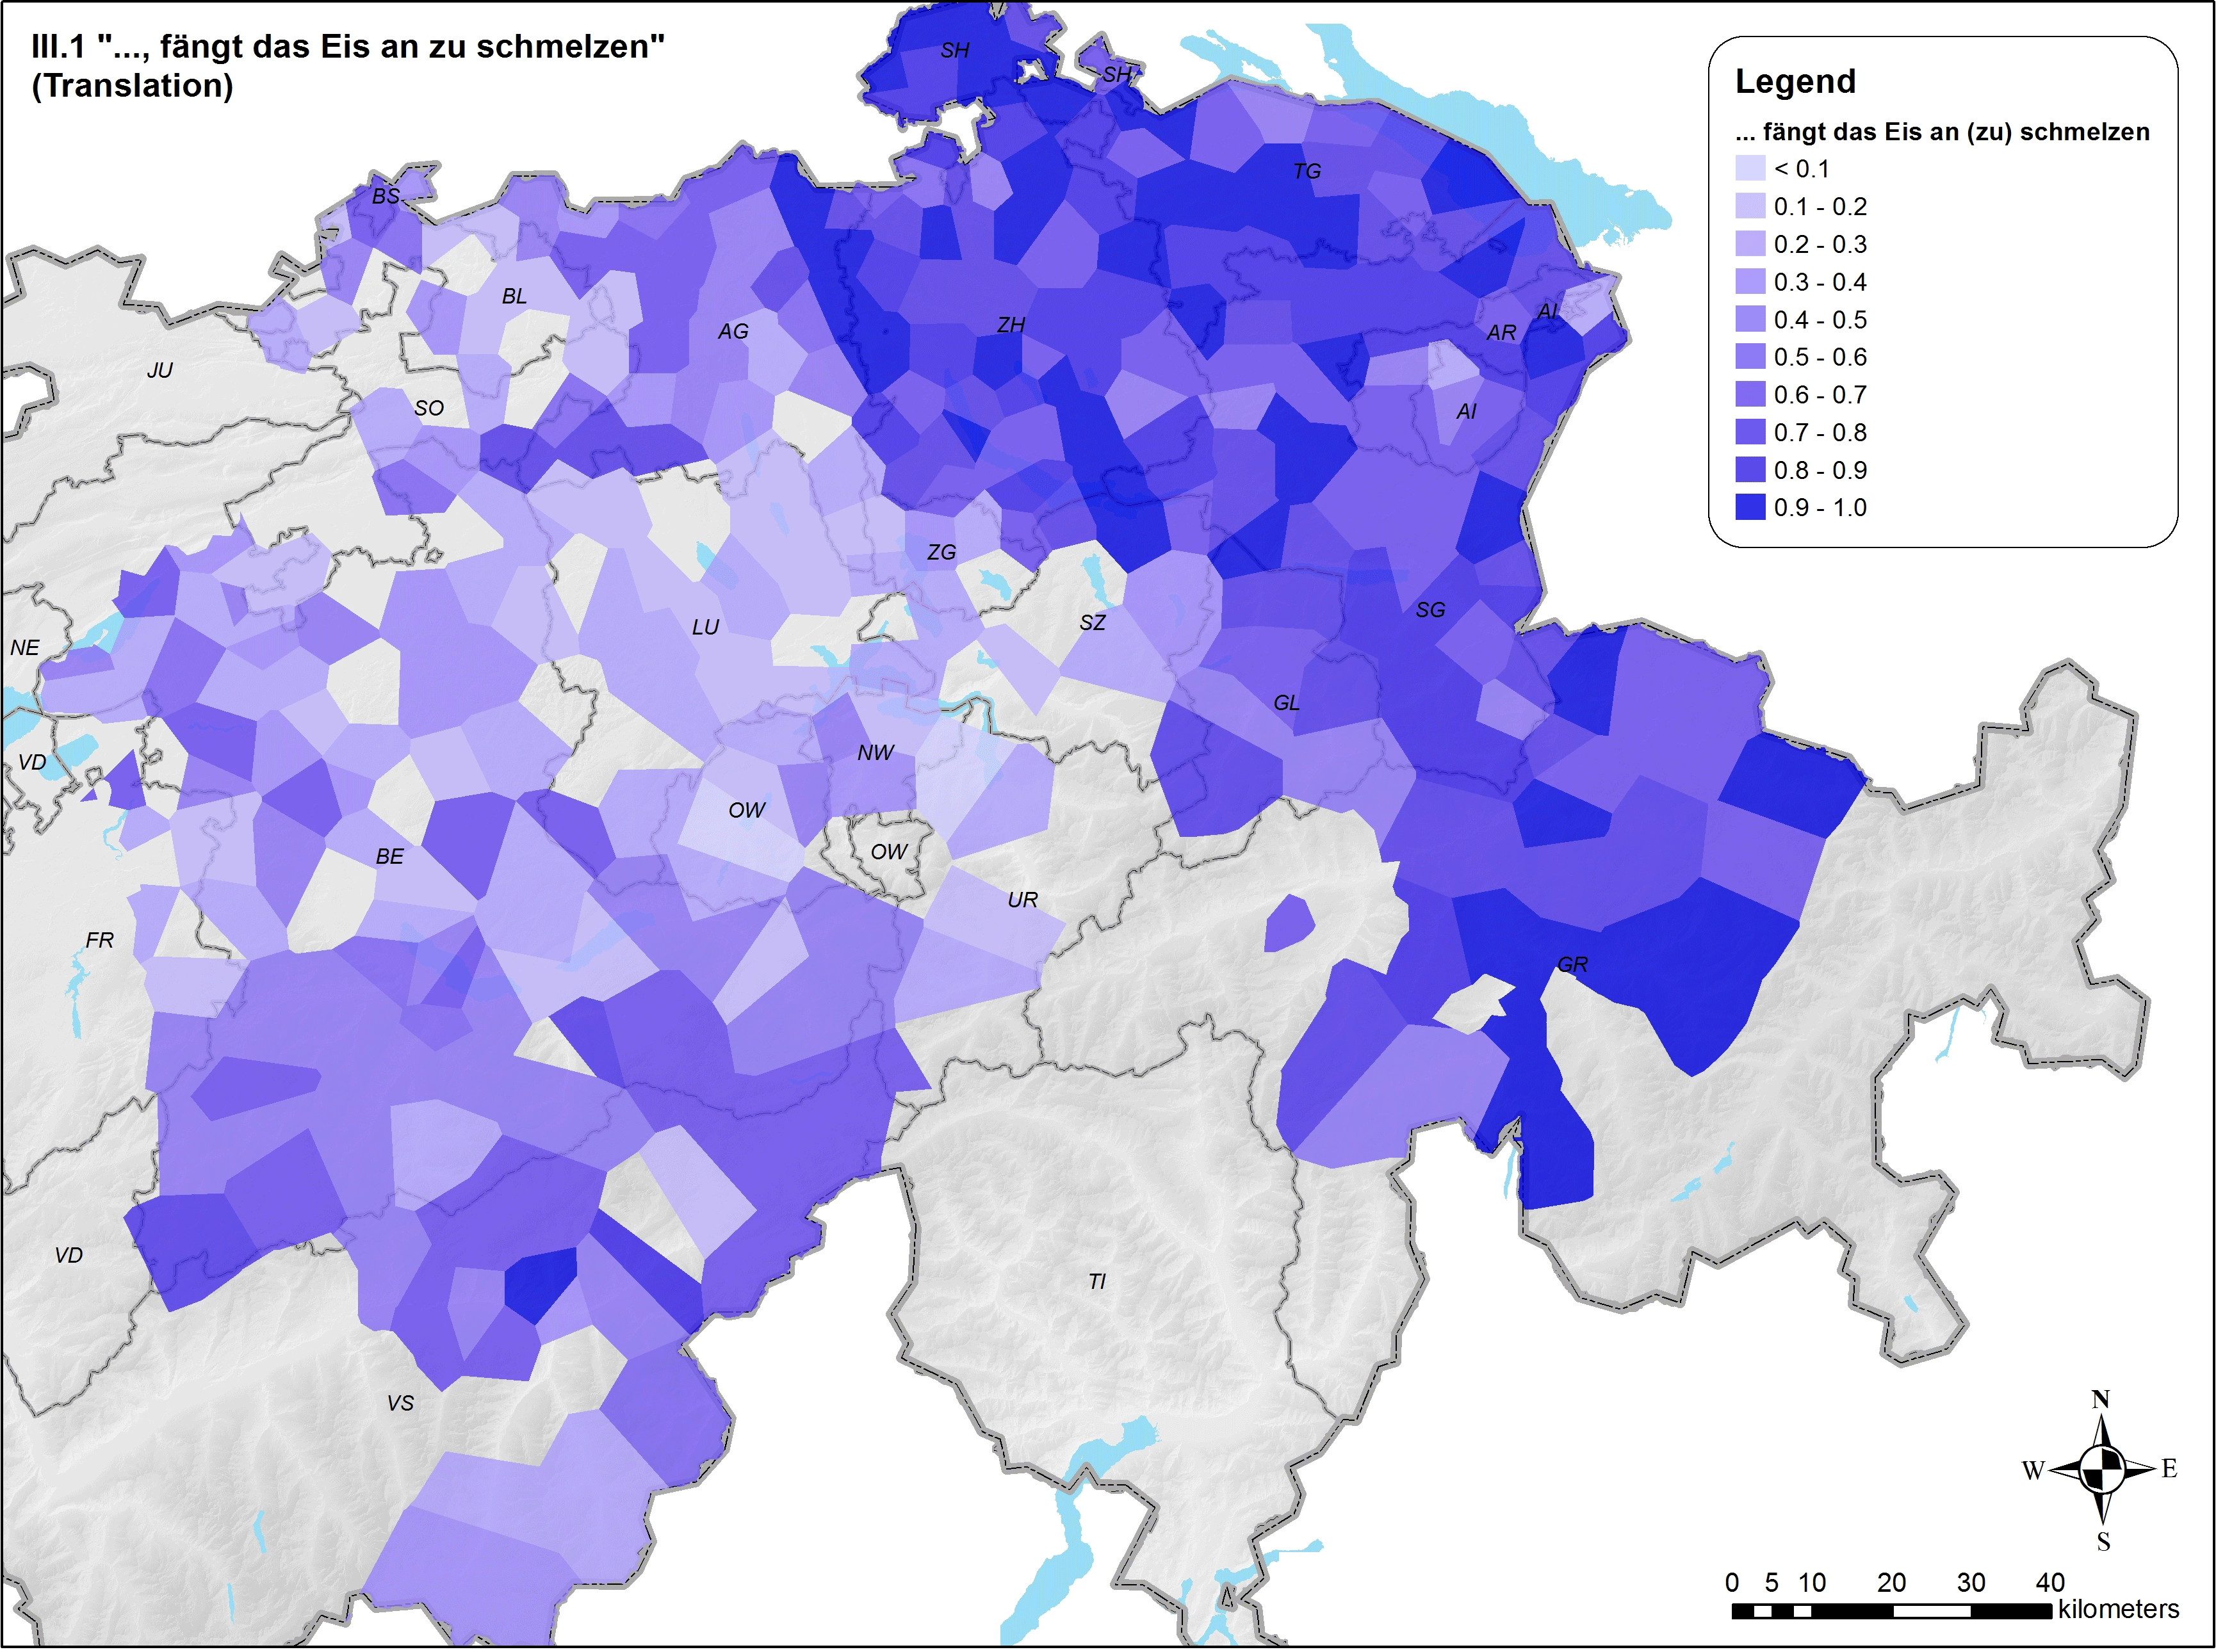
\includegraphics[width=\textwidth]{illustrations/stoeck_fig1}
\label{fig:1}
\caption{Geographical distribution of the variant \emph{… fängt das Eis an (zu) schmelzen}.}
\end{figure}

The different color hues indicate the percentage of informants at each place who provided the respective translation in the questionnaire. As the map suggests, the form is clearly dominant in the eastern part of Switzerland where we find an agreement of almost 100\% of informants in many locations. Moreover, the map shows that the variant seems to be used almost all over the research area apart from some locations in the center and in the west. For a comparison we will consider the distribution of the variant \emph{... fängt das Eis }\emph{\textsc{afa}}\emph{ schmelzen} which is displayed in \figref{fig:2}.

  
\begin{figure}
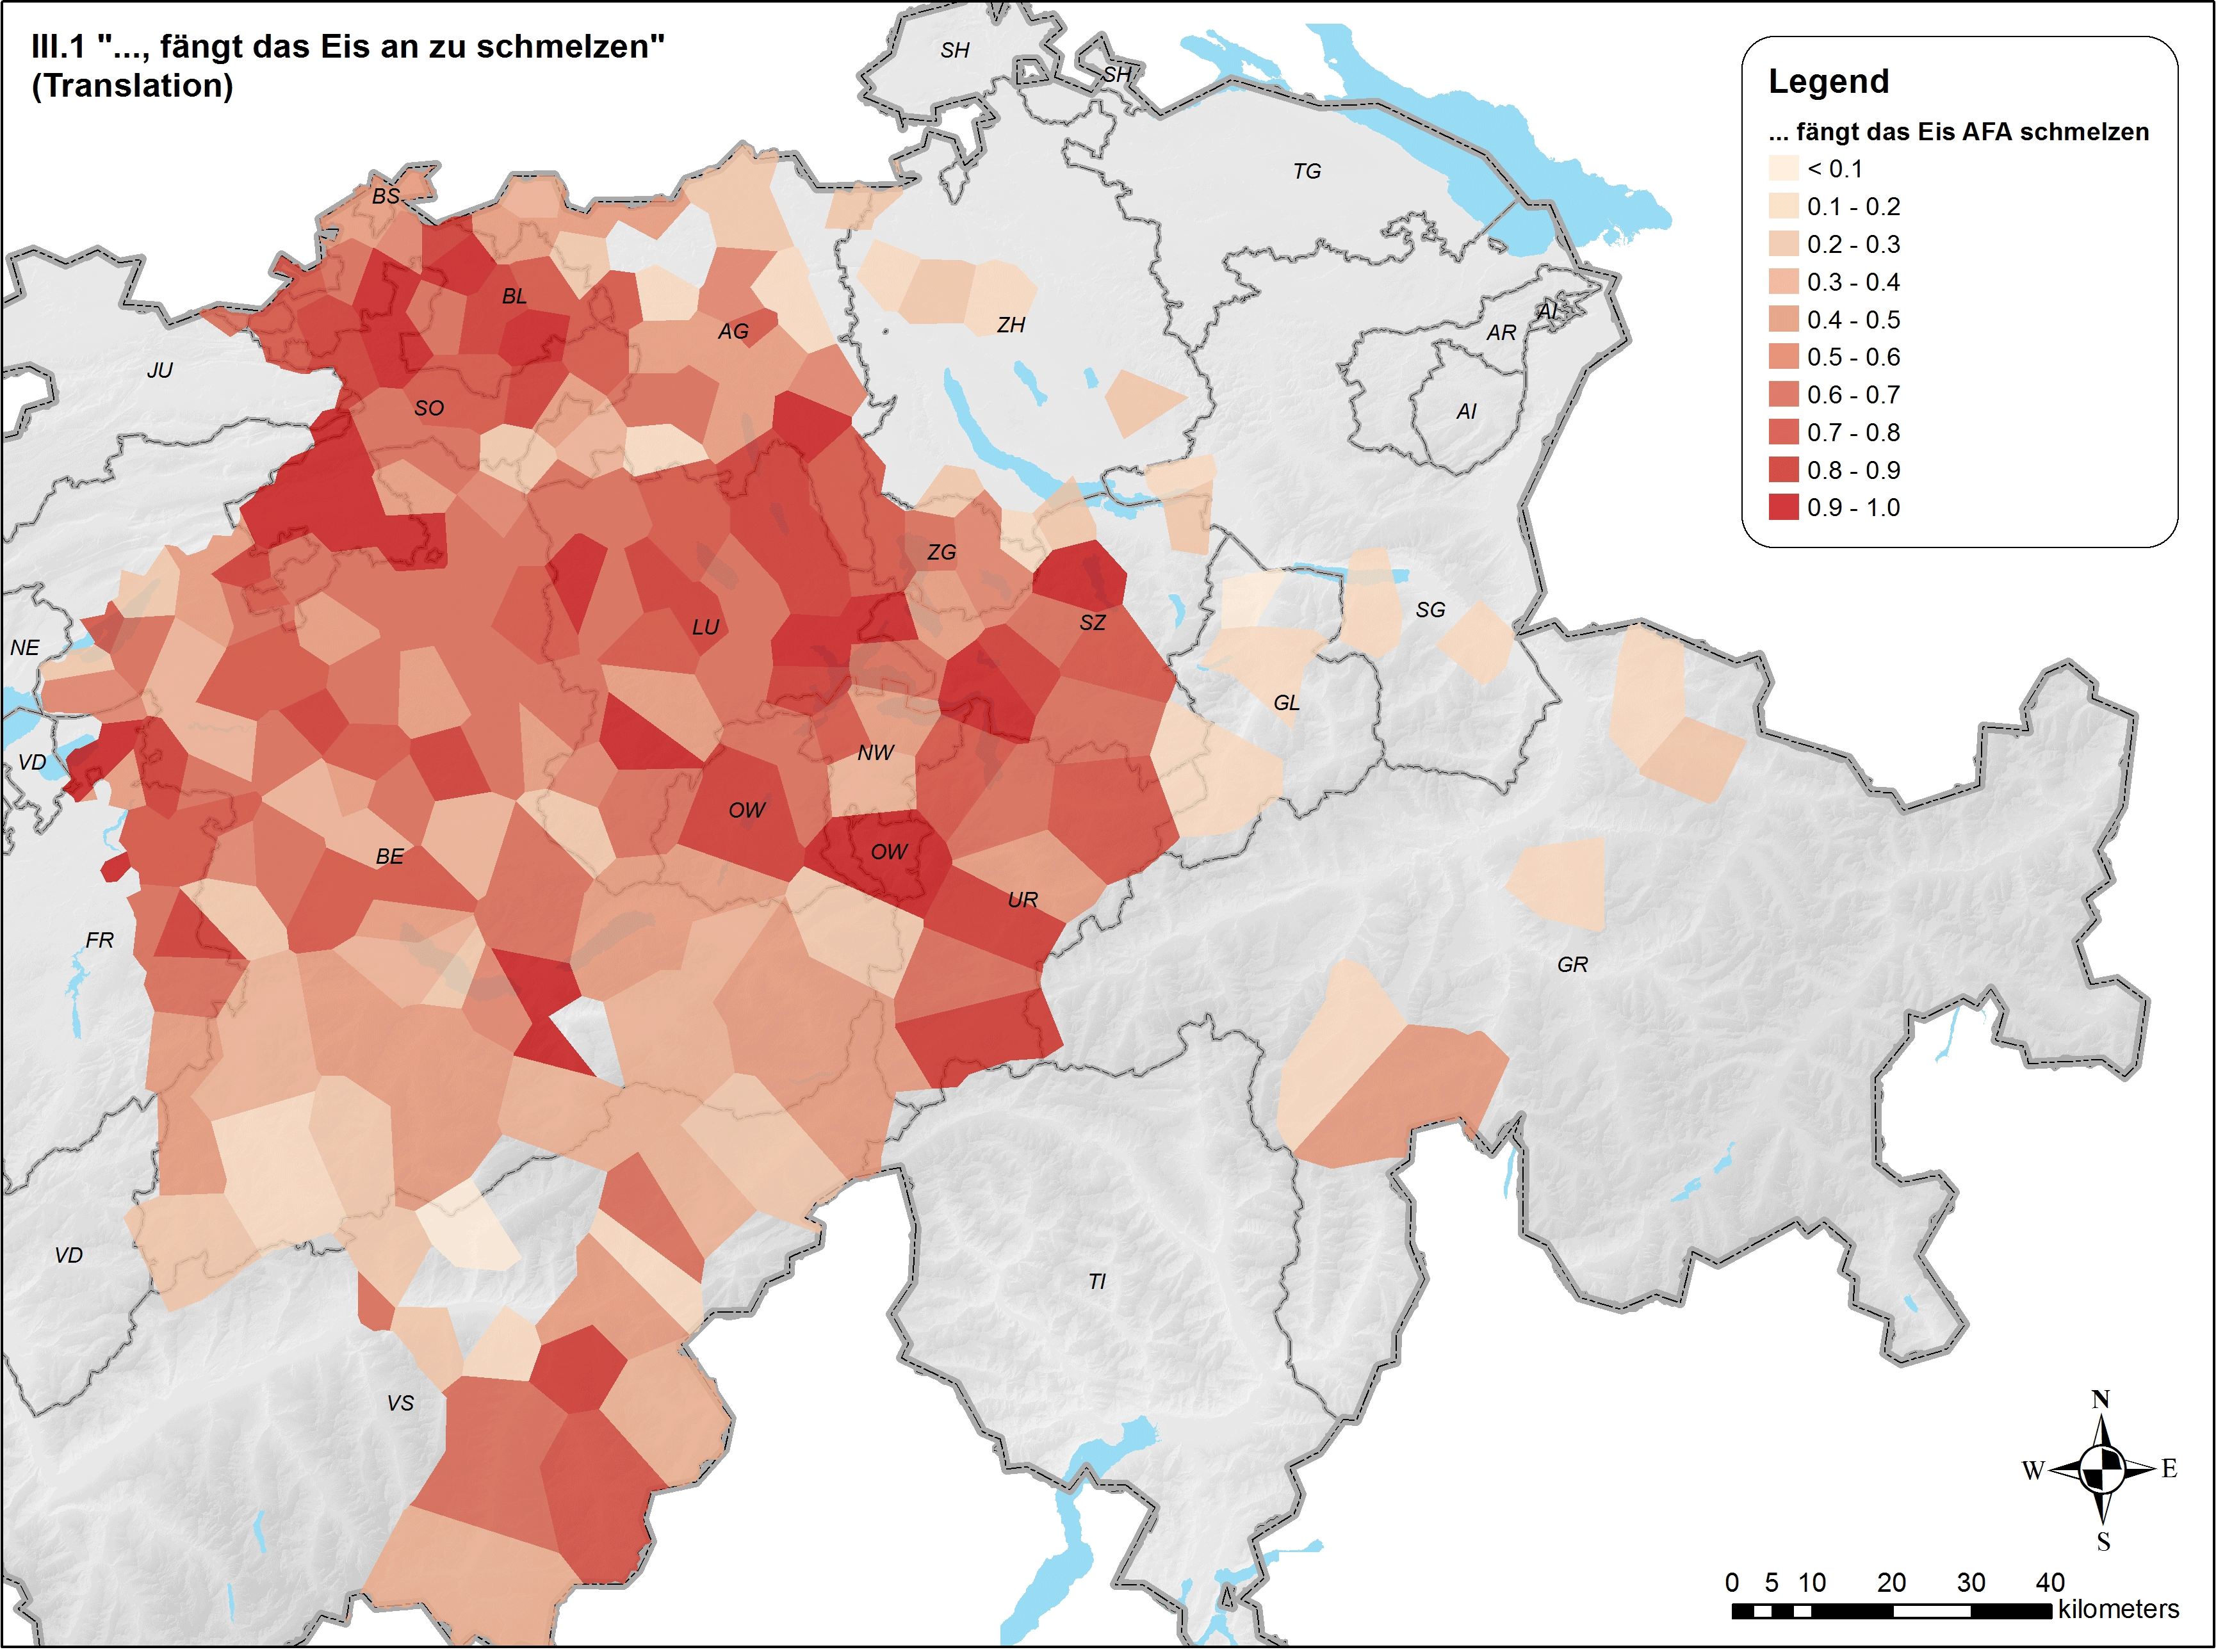
\includegraphics[width=\textwidth]{illustrations/stoeck_fig2}
\label{fig:2}
\caption{Geographical distribution of the variant \emph{… fängt das Eis \textsc{afa} schmelzen}.}
\end{figure}
 
As for the \textsc{afa} variant, we can observe a concentration in the center and (north)western parts of Switzerland, while it is not used at all in the east. A direct comparison of Figures 1 and 2 reveals that in large parts of German-speaking Switzerland – especially center and west – both variants can be observed, whereas particularly in the east just one variant seems to be used exclusively. At this point we have gained a very precise idea of the distributions of the two variants separately. However, it is difficult to tell what their relationship looks like, especially in the areas where both variants are used. For this purpose I combined both variants on a single map (\figref{fig:3}), the dominant variant, i.e. the variant that was provided by the most informants, at each location.
 
\begin{figure}
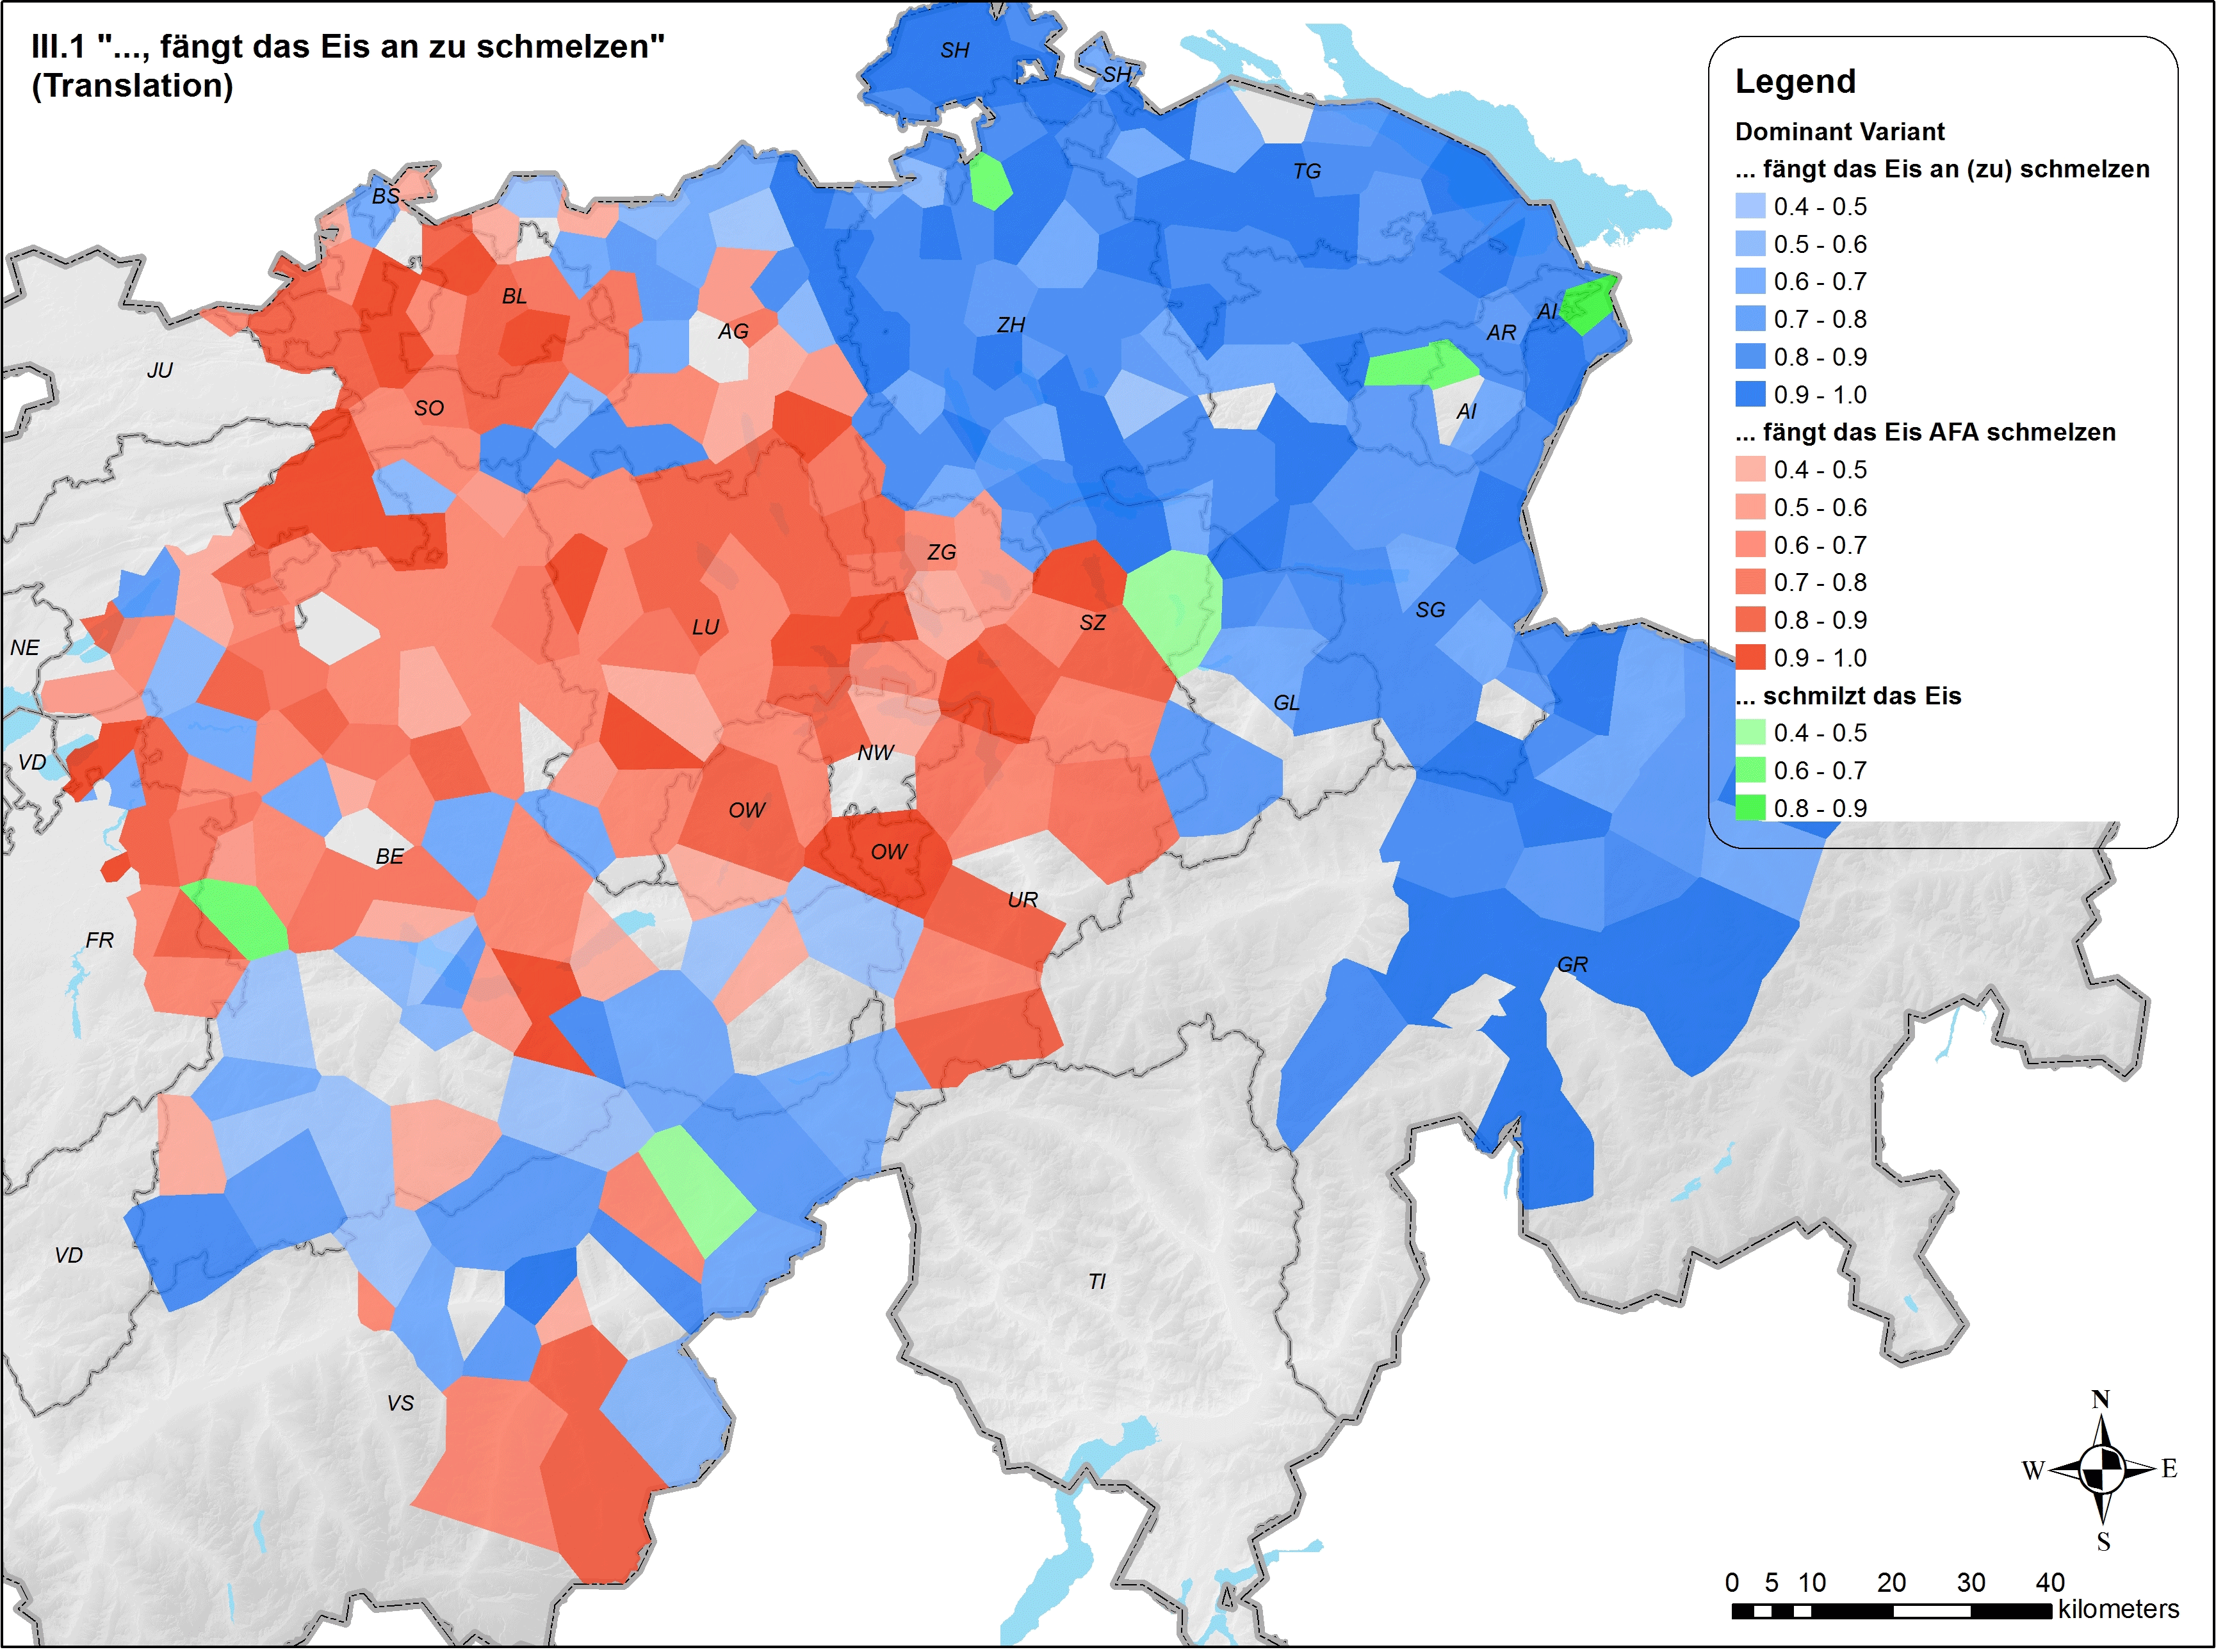
\includegraphics[width=\textwidth]{illustrations/stoeck_fig3}
\label{fig:3}
\caption{Geographic distribution of the dominant variants.}
\end{figure}

Four things can be observed in \figref{fig:3}: First, the dominant variants do not seem to be distributed randomly, rather they seem to shape areas. Especially in the central and (north-)western parts of Switzerland it becomes clear that the variant \emph{... fängt das Eis }\emph{\textsc{afa}}\emph{ schmelzen} appears to be the predominant form – an observation that could hardly be made by regarding the individual maps. Second, the variant \emph{... schmilzt das Eis} (‘the ice melts’) is dominant in only seven scattered locations, although a separate look at its geographic distribution reveals that it can be found in almost all parts of the research area. Third, some of the polygons are ‘empty’, i.e. none of the variants could be assigned to them. This is due to the fact that in these locations no single variant turned out to be dominant, but instead two forms were used by equal numbers of informants.

The fourth –  and in this context most important –  point regards the percentage values of the dominant variants. If our goal was, like in many ‘traditional’ approaches, to determine one form for each location, the most obvious procedure would be to choose the dominant variant. This way we would obtain a more or less clear east-west division of our research area with some exceptions in the southern Bernese (\textsc{be}) area\footnote{The cantons are indicated by two-letter codes. In the case of the canton Bern, the code is \textsc{be}.} and the canton of Wallis (‘Valais’, \textsc{vs}). However, if we take the percentage values of the dominant variants into account, it becomes obvious that this division would hide a lot of the linguistic reality. While in some locations we find very high rates of agreement, in other places the highest values for the dominant variant range between only 40 and 50 percent. This means that there must be at least two or three (or even more) different forms given as translations by the informants.

If we abstract away from the variants themselves and only consider the agreement rate of the dominant variant at each location, we obtain a visualization as depicted in \figref{fig:4}. As the map shows, the agreement between the informants seems to be generally higher in the northern and eastern regions (at least for this question), whereas especially in the southern parts of the canton Bern (\textsc{be}) there is very little agreement, i.e. comparatively, the informants differ greatly in their answers.
  
\begin{figure}
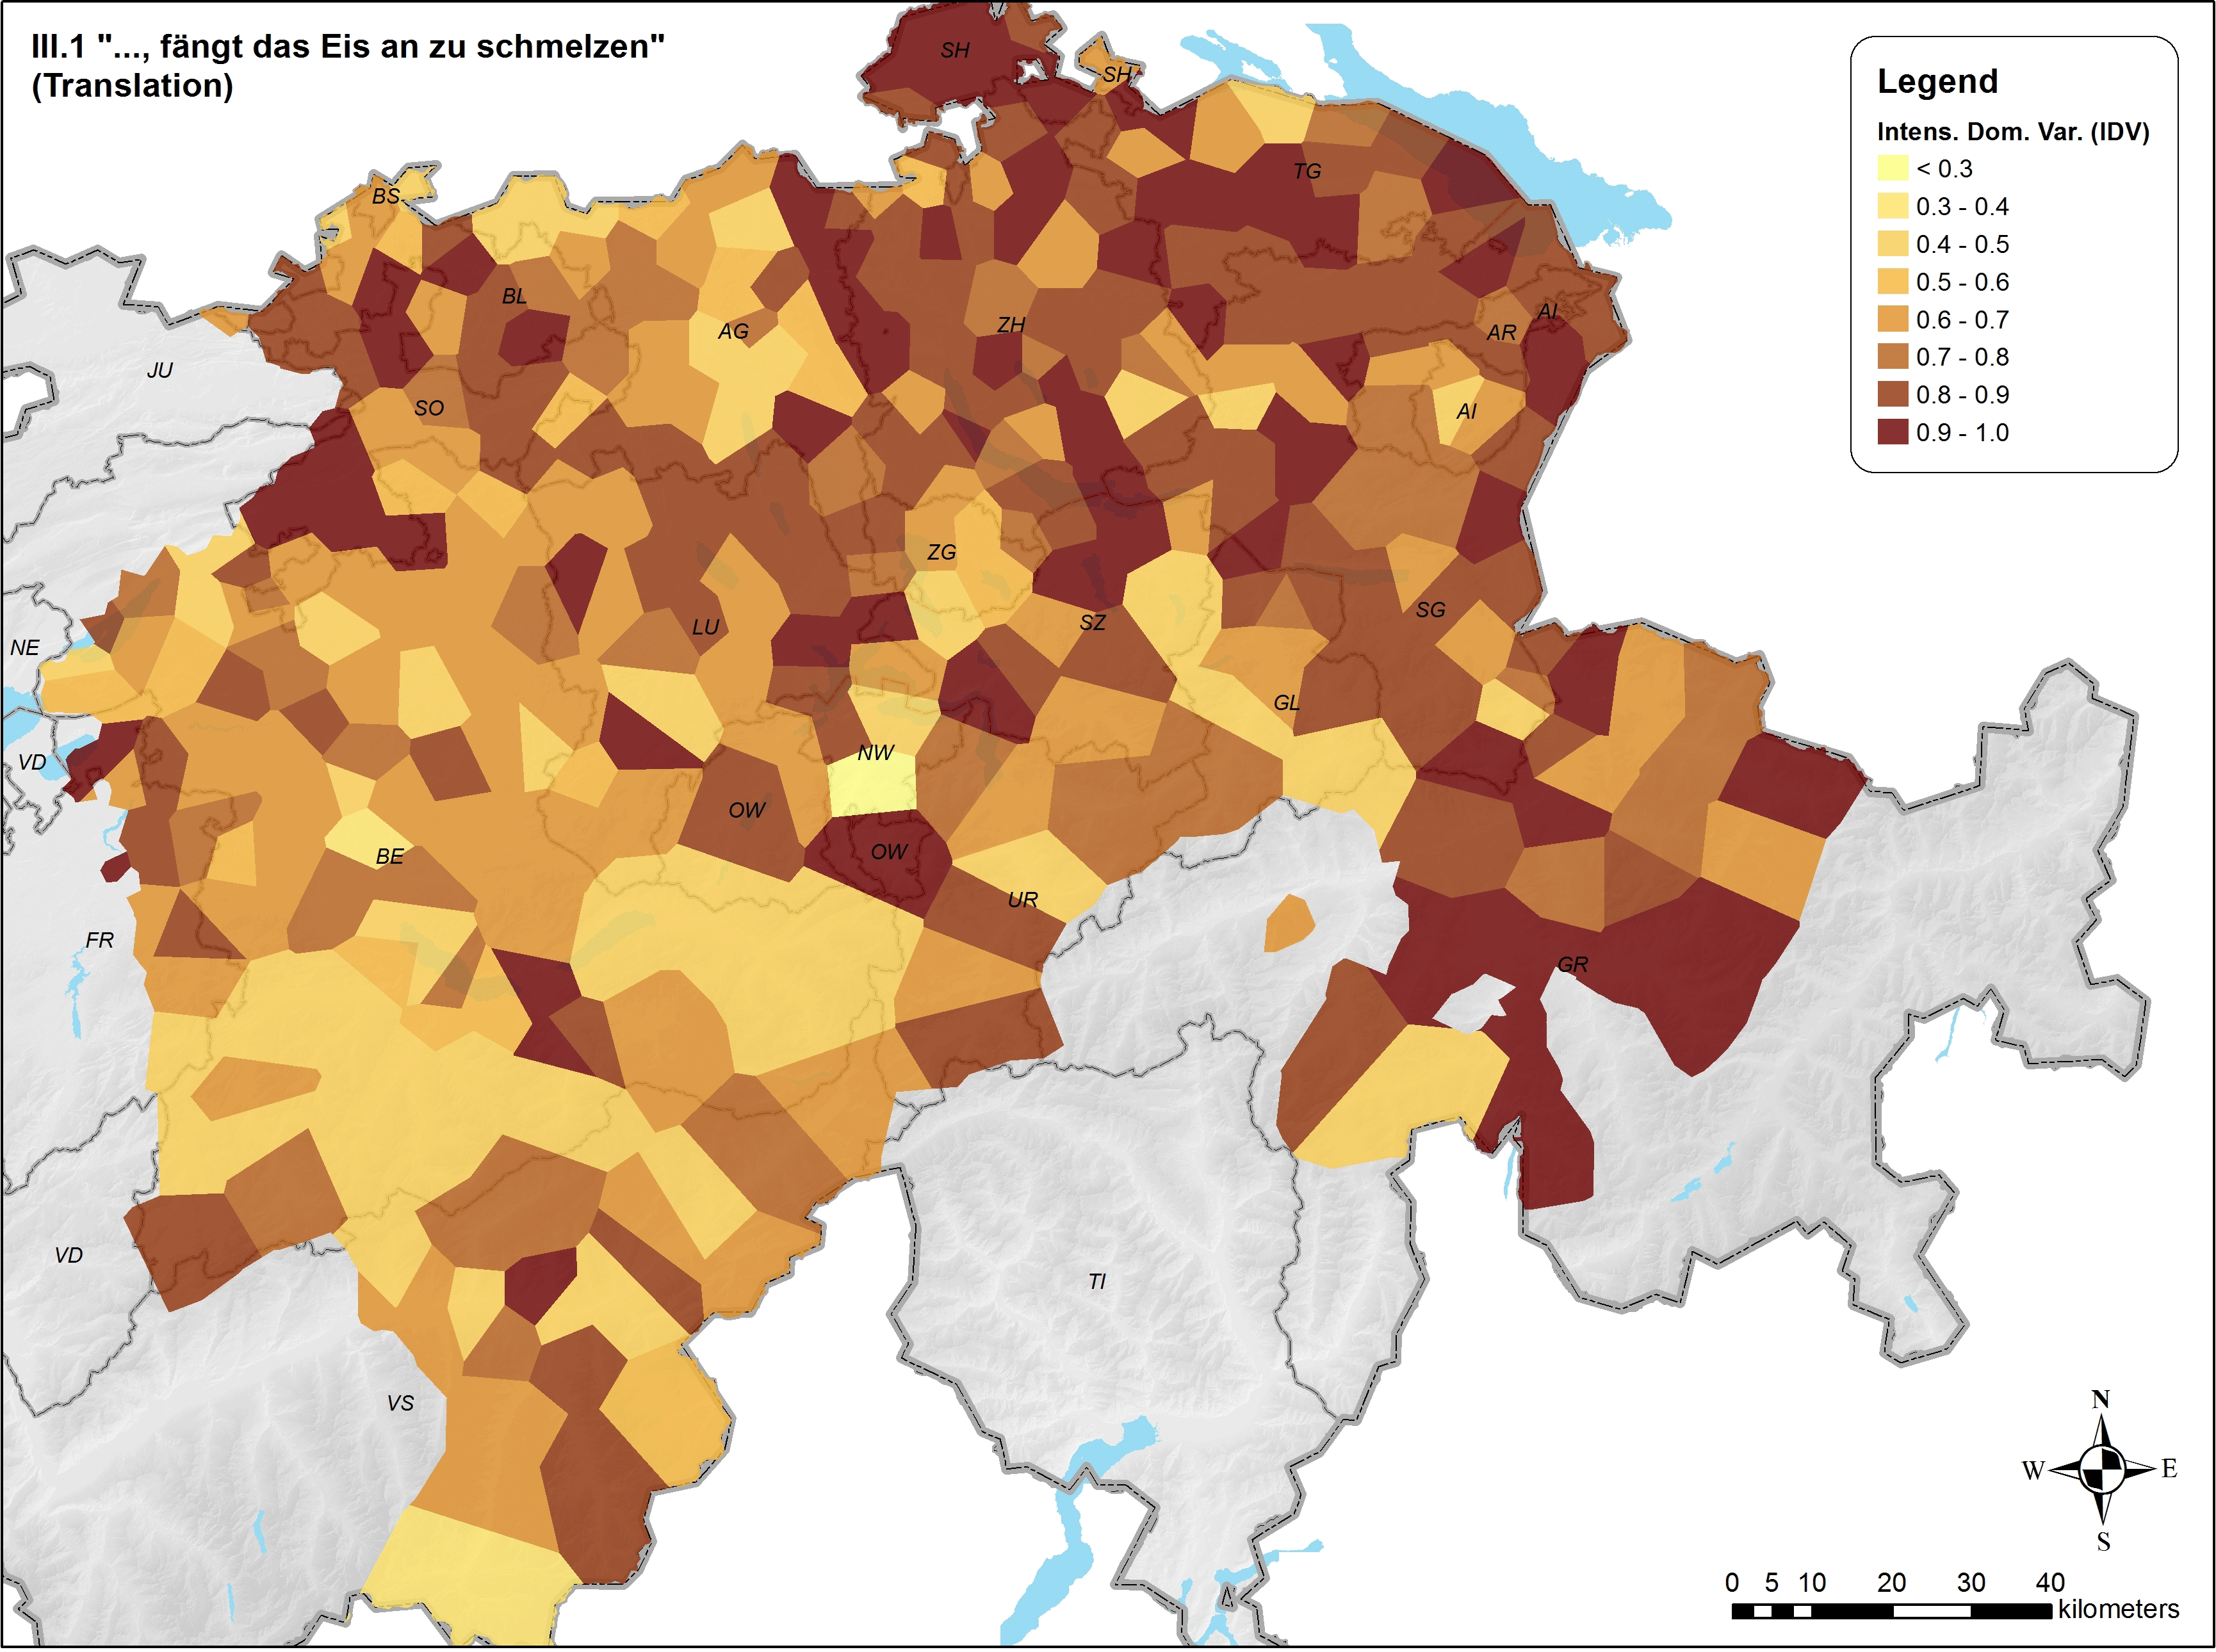
\includegraphics[width=\textwidth]{illustrations/stoeck_fig4}
\label{fig:4}
\caption{Intensity of the dominant variant.}
\end{figure}
 
The analysis of this single phenomenon has shown that variation turns out to be very frequent once multiple informants are taken into account at one location. It also became obvious that in spite of all the variation, the geographic distribution of the different variants is not random but shows a rather characteristic pattern.\footnote{ Of course, this could be subject to further geostatistical testing.} As a consideration of more and different phenomena from the SADS shows,\footnote{ Examples of which would be word order variation in verb clusters (e.g. \emph{… ob er einmal heiraten will} vs. \emph{… ob er einmal will heiraten}, ‘… whether he ever wants to get married’; \citealt{seiler_three_2004}) or prepositional dative marking (e.g. \emph{Das gehört an/in meiner Schwester} vs. \emph{Das gehört meiner Schwester}, ‘It belongs to my sister’; \citealt{seiler_prapositionale_2003}).} the observations made in this section do not hold only for this phenomenon but can be generalized for most syntactic variables. Although the geographic patterns are not always the same, some areas seem to display more variation than others. The goal of the following part will be to classify the research area into regions with respect to inter-speaker variation.

\section{Variation Index}

As the observations in the previous section have shown, the percentage of agreement between the informants regarding the dominant variant can be taken as an indicator for variation. If, for example, we find 100 percent agreement, this means that all informants gave the same answer and that there is, therefore, no variation at all. Agreement rates between 50 and 100 percent mean that there must be two variants (or more), agreement rates of less than 50 per cent point to at least three variants, and so on. Of course these percentage values do not provide information about the exact number of variants,\footnote{ It should be noted that the total number of variants per phenomenon differs between two and eight. Although a higher total number does not automatically imply a higher inter-speaker variation at the individual locations (the different variants could theoretically be used in separate locations), this fact should be taken into account in a detailed analysis of the variability of the different phenomena. However, since we are primarily interested in the geographic distribution of inter-speaker variation, we can neglect these differences here.} but they can give us an idea about variation in the following sense:

\begin{itemize}
\item high value \textasciitilde ~high agreement \textasciitilde ~little variation
\item low value \textasciitilde ~little agreement \textasciitilde ~much variation
\end{itemize}

In order to classify the research area according to the inter-speaker syntactic variation at the individual survey locations, it will be necessary to quantify the agreement rates including multiple phenomena. At the present time not all questions which were part of the SADS survey have been edited completely, so that their inclusion in the analyses might have been problematic. Therefore a subset of 57 questions from the SADS comprising 26 different syntactic phenomena was chosen as data for the analyses. As a simple mathematical measure of quantification the arithmetic mean of all agreement rates for each location was calculated. We will call it \emph{agreement index}, and it is defined as follows:\footnote{I am aware that the arithmetic mean is a very simple statistic measure which does not necessarily have to be quoted as mathematical formula. Nevertheless, it shall be presented here so that it is easier in the remainder of the article to refer to its elements. }

\begin{equation}
\mathit{AI}=\frac{1}{n}\sum _{i=1}^{n}{{\mathit{IDV}}_{i}}
\end{equation}

where

\begin{itemize}
\item \emph{IDV} stands for the \emph{intensity of the dominant variant} (i.e. the agreement rate between those informants providing the dominant variant as \emph{their} variant),

\item each \emph{i} stands for an individual question from the SADS,

\item \emph{n} is the total number of SADS questions taken into account.

\item Since our main focus is on variation rather than agreement and we would, therefore, like to obtain higher values for more variation and smaller values for less variation (and all values range between 0 and 1), we define our \emph{variation index} as\\
\begin{equation}
\mathit{VI}=1-\mathit{AI}
\end{equation}
\end{itemize}

For a first impression of the geographic distribution, the variation indices are mapped to the SADS survey points, the result of which is displayed in \figref{fig:5}.

\begin{figure}
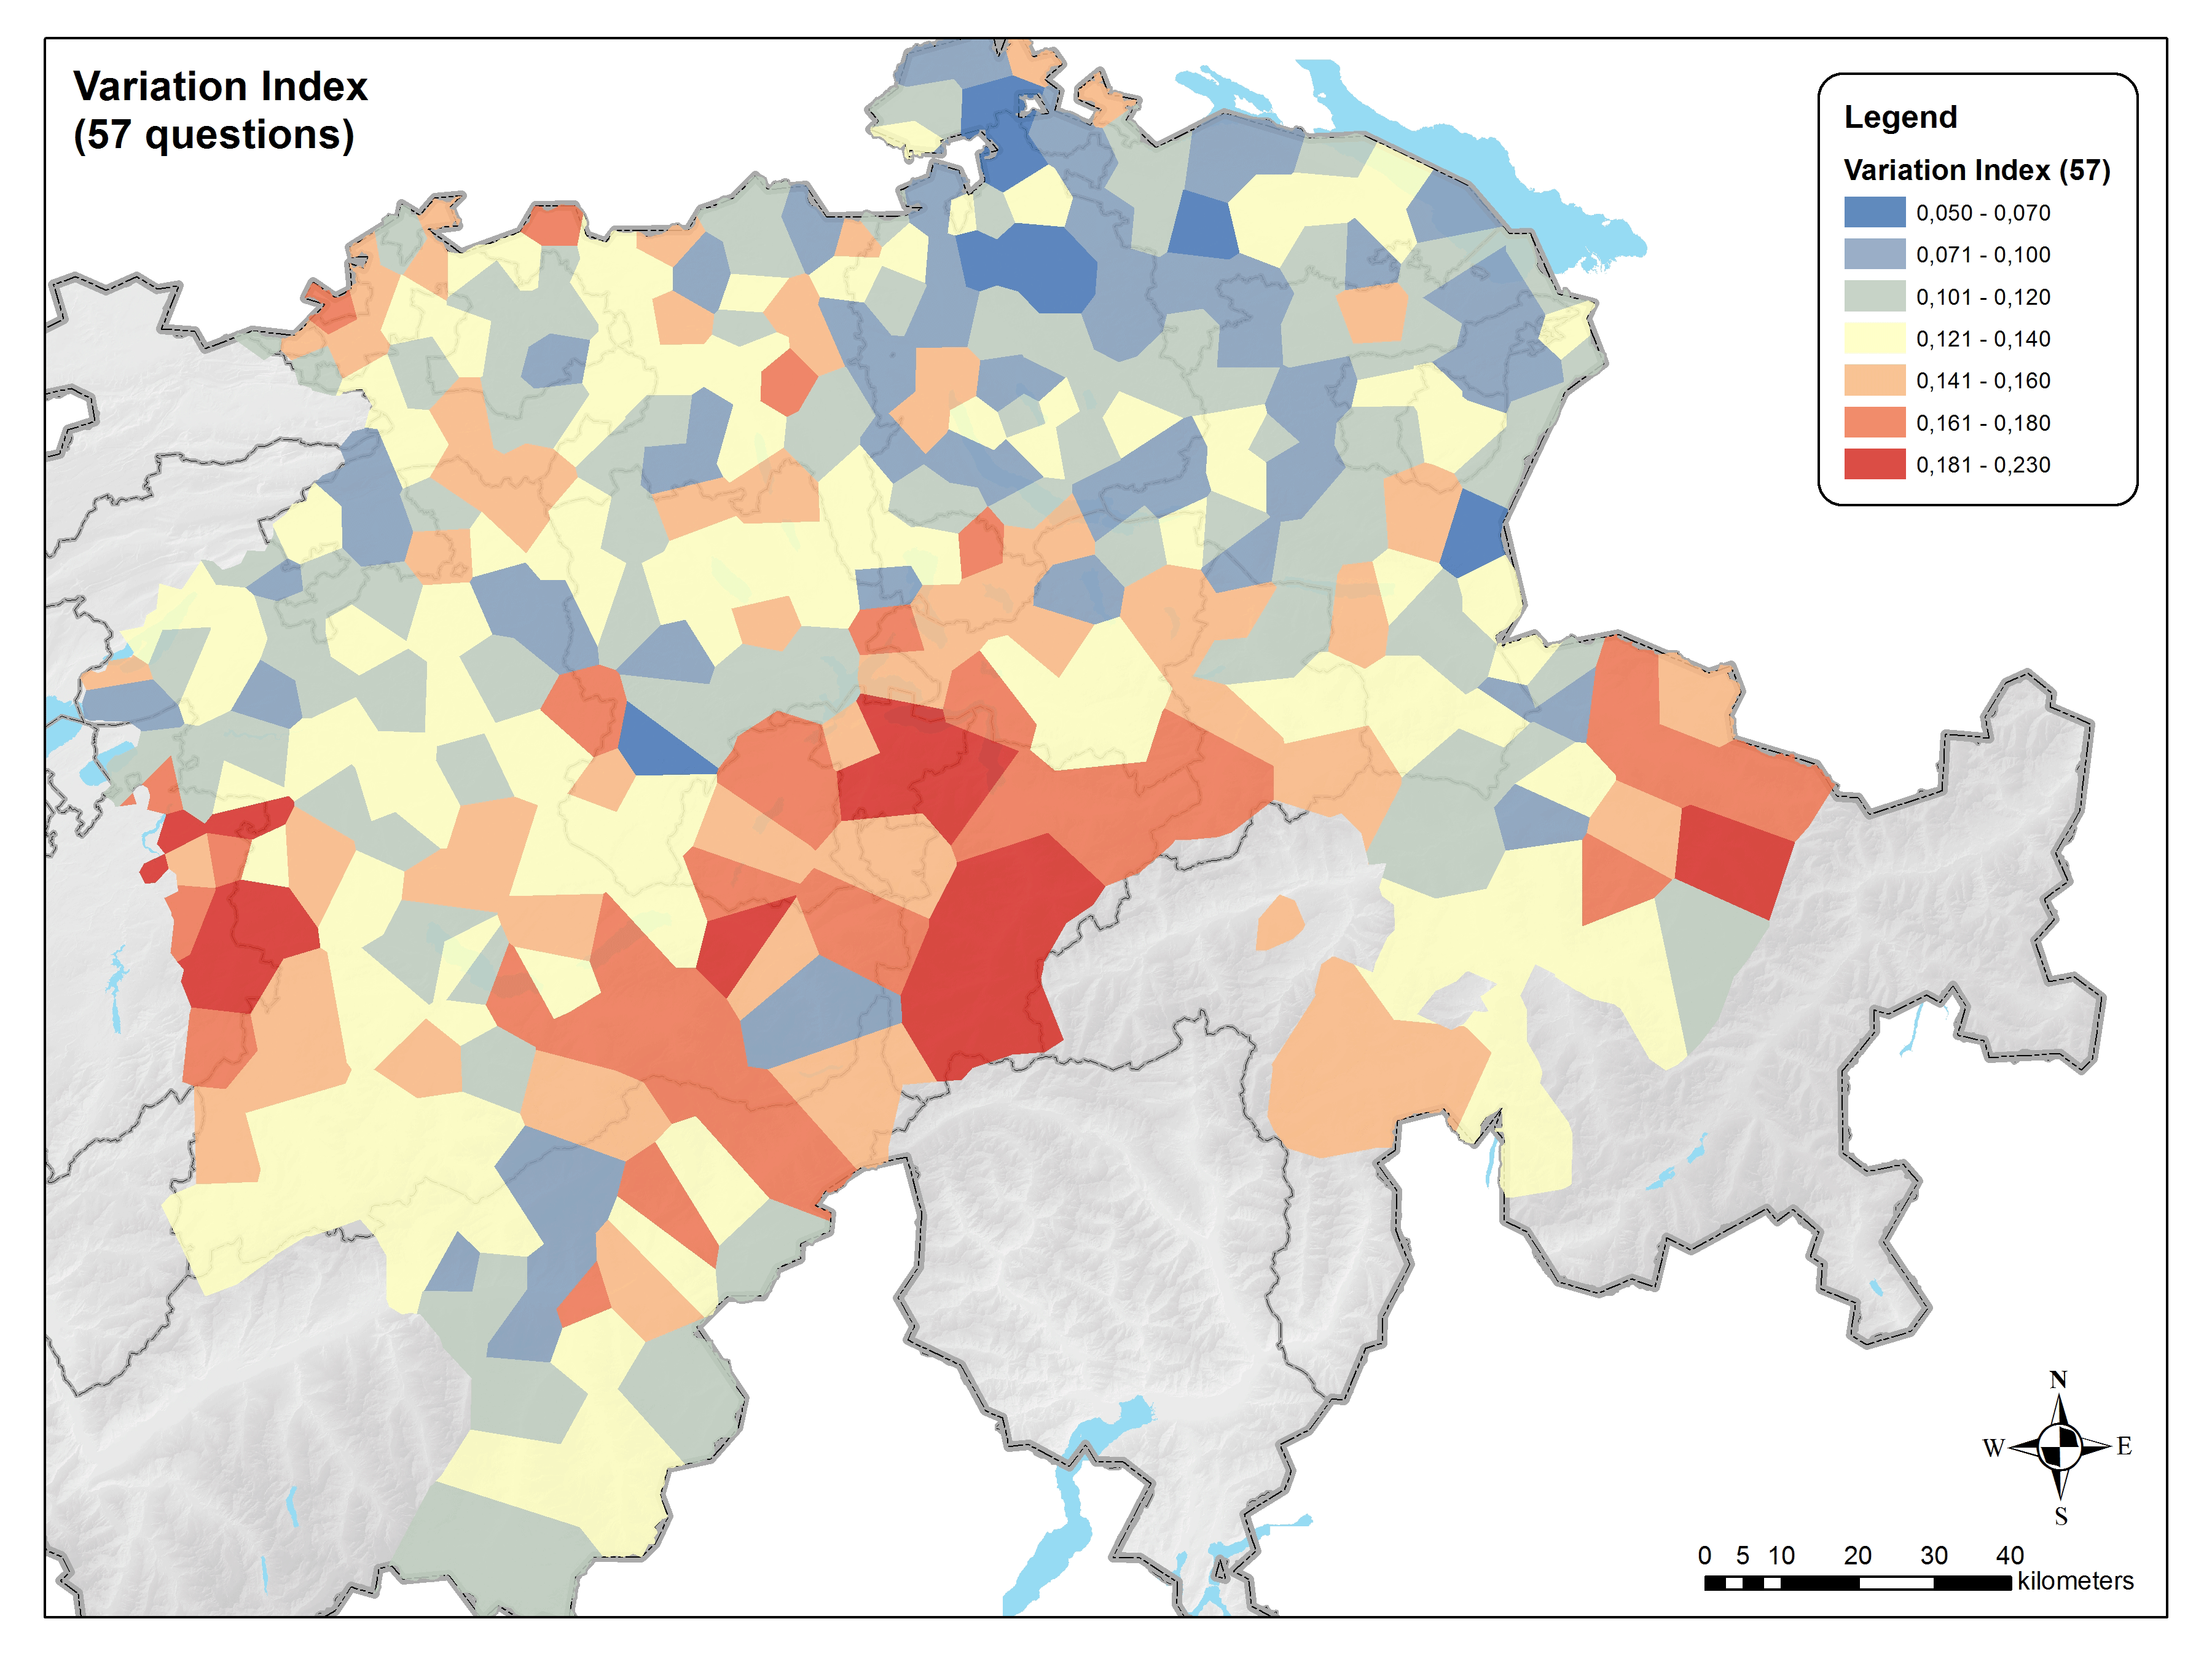
\includegraphics[width=\textwidth]{illustrations/stoeck_fig5}
\label{fig:5}
\caption{Geographic mapping of the \emph{variation index} including 57 SADS questions.}
\end{figure}

The different colors indicate different degrees of variation (or agreement between the informants, respectively). Red colors stand for a high variation index, blue colors for low values. At first glance the pattern seems a bit fuzzy, but there are some concentrations of high and low variation observable. While in the north-east there are many blue and almost no red areas, the central part of Switzerland especially shows a clear concentration of high values. Moreover, there seem to be red clusters at the very western (canton of Fribourg, \textsc{fr}) and eastern (canton of Grisons, \textsc{gr}) borders. Although \figref{fig:5} provides a general impression of the geographical pattern of syntactic variation, two questions remain:

\begin{enumerate}
\item To what degree is the variation index as displayed in \figref{fig:5} a result of the choice of the SADS questions that were taken into account? Would the geographical pattern look different if we had used a different set of variables?
\item How much is our interpretation of \figref{fig:5} influenced by intuition? Are there more elaborate ways to (statistically) confirm the observed geographical pattern, i.e. to obtain more robust results?
\end{enumerate}

Let us first address question number two. In geography, questions of this type are addressed with the concept of spatial autocorrelation, “a measure of spatial dependency that quantifies the degree of spatial clustering or dispersion in the values of a variable measured across a set of locations” \citep[34]{grieve_use_2011}. In our case, the variable is the variation index with its different values at the different SADS survey locations. If we assume that in some parts of our research area there are clusters of polygons with similar colors (and thus similar values), we should expect a positive autocorrelation in these parts.\footnote{For a more detailed description of spatial autocorrelation and its application to SADS data cf. \citet[62--63]{sibler_visualisierung_2011}.} Generally there are two types of spatial autocorrelation statistics: “global measures [which] identify whether the values of a variable exhibit a significant overall pattern of regional clustering”, and “local measures [which] identify the location of significant high and low value clusters” \citep[34]{grieve_use_2011}. While both methods have been applied to our data, for illustration purposes I will focus on the latter type in order to determine so-called \emph{hot} and \emph{cold} spots. For this purpose I used the Hot Spot Analysis tool in ArcGIS, which uses the Getis-Ord Gi* statistic \citep{getis_analysis_1992}.

\begin{quote}[It] works by looking at each feature within the context of neighboring features. A feature with a high value is interesting but may not be a statistically significant hot spot. To be a statistically significant hot spot, a feature will have a high value and be surrounded by other features with high values as well.\footnote{For the exact reference cf. the ArcGIS online help “How Hot Spot Analysis (Getis-Ord Gi*) works”: \url{http://resources.arcgis.com/en/help/main/10.2/index.html\#/How\_Hot\_Spot\_Analysis\_Getis\_Ord\_Gi\_works/005p00000011000000/} [accessed November 2014]}(ESRI 2014)
\end{quote}

As a result, for each location the analysis yields a z-score and a p-value, both of which are associated with standard normal distribution. Very high positive z-scores indicate a clustering of values which are higher than the mean value, thus building a hot spot \citep[65]{sibler_visualisierung_2011}. In the case of our data the VI for every survey location is compared with all other VIs within a distance of 17.4km, a value computed automatically to ensure that each location has at least one neighbor. If a location has a very high positive VI and the locations within the defined radius also have high VIs, it becomes part of a hot spot. In the opposite case (i.e. high negative values) we find a cold spot. \figref{fig:6} displays the results mapped to the SADS survey locations in order to identify the hot and cold spots geographically.
%]{
As a result, for each location the analysis yields a z-score and a p-value, both of which are associated with standard normal distribution. Very high positive z-scores indicate a clustering of values which are higher than the mean value, thus building a hot spot \citep[65]{sibler_visualisierung_2011}. In the case of our data the \emph{VI} for every survey location is compared with all other \emph{VI}s within a distance of 17.4km, a value computed automatically to ensure that each location has at least one neighbor.\footnote{The requirement of having at least one neighbor to be included in the analysis is especially important for the locations in the periphery. On average, there are twelve neighbors included within the radius of 17.4km for each location.} If a location has a very high positive \emph{VI} and the locations within the defined radius also have high \emph{VI}s, it becomes part of a hot spot. In the opposite case (i.e. high negative values) we find a cold spot. \figref{fig:6} displays the results mapped to the SADS survey locations in order to identify the hot and cold spots geographically.

\begin{figure}
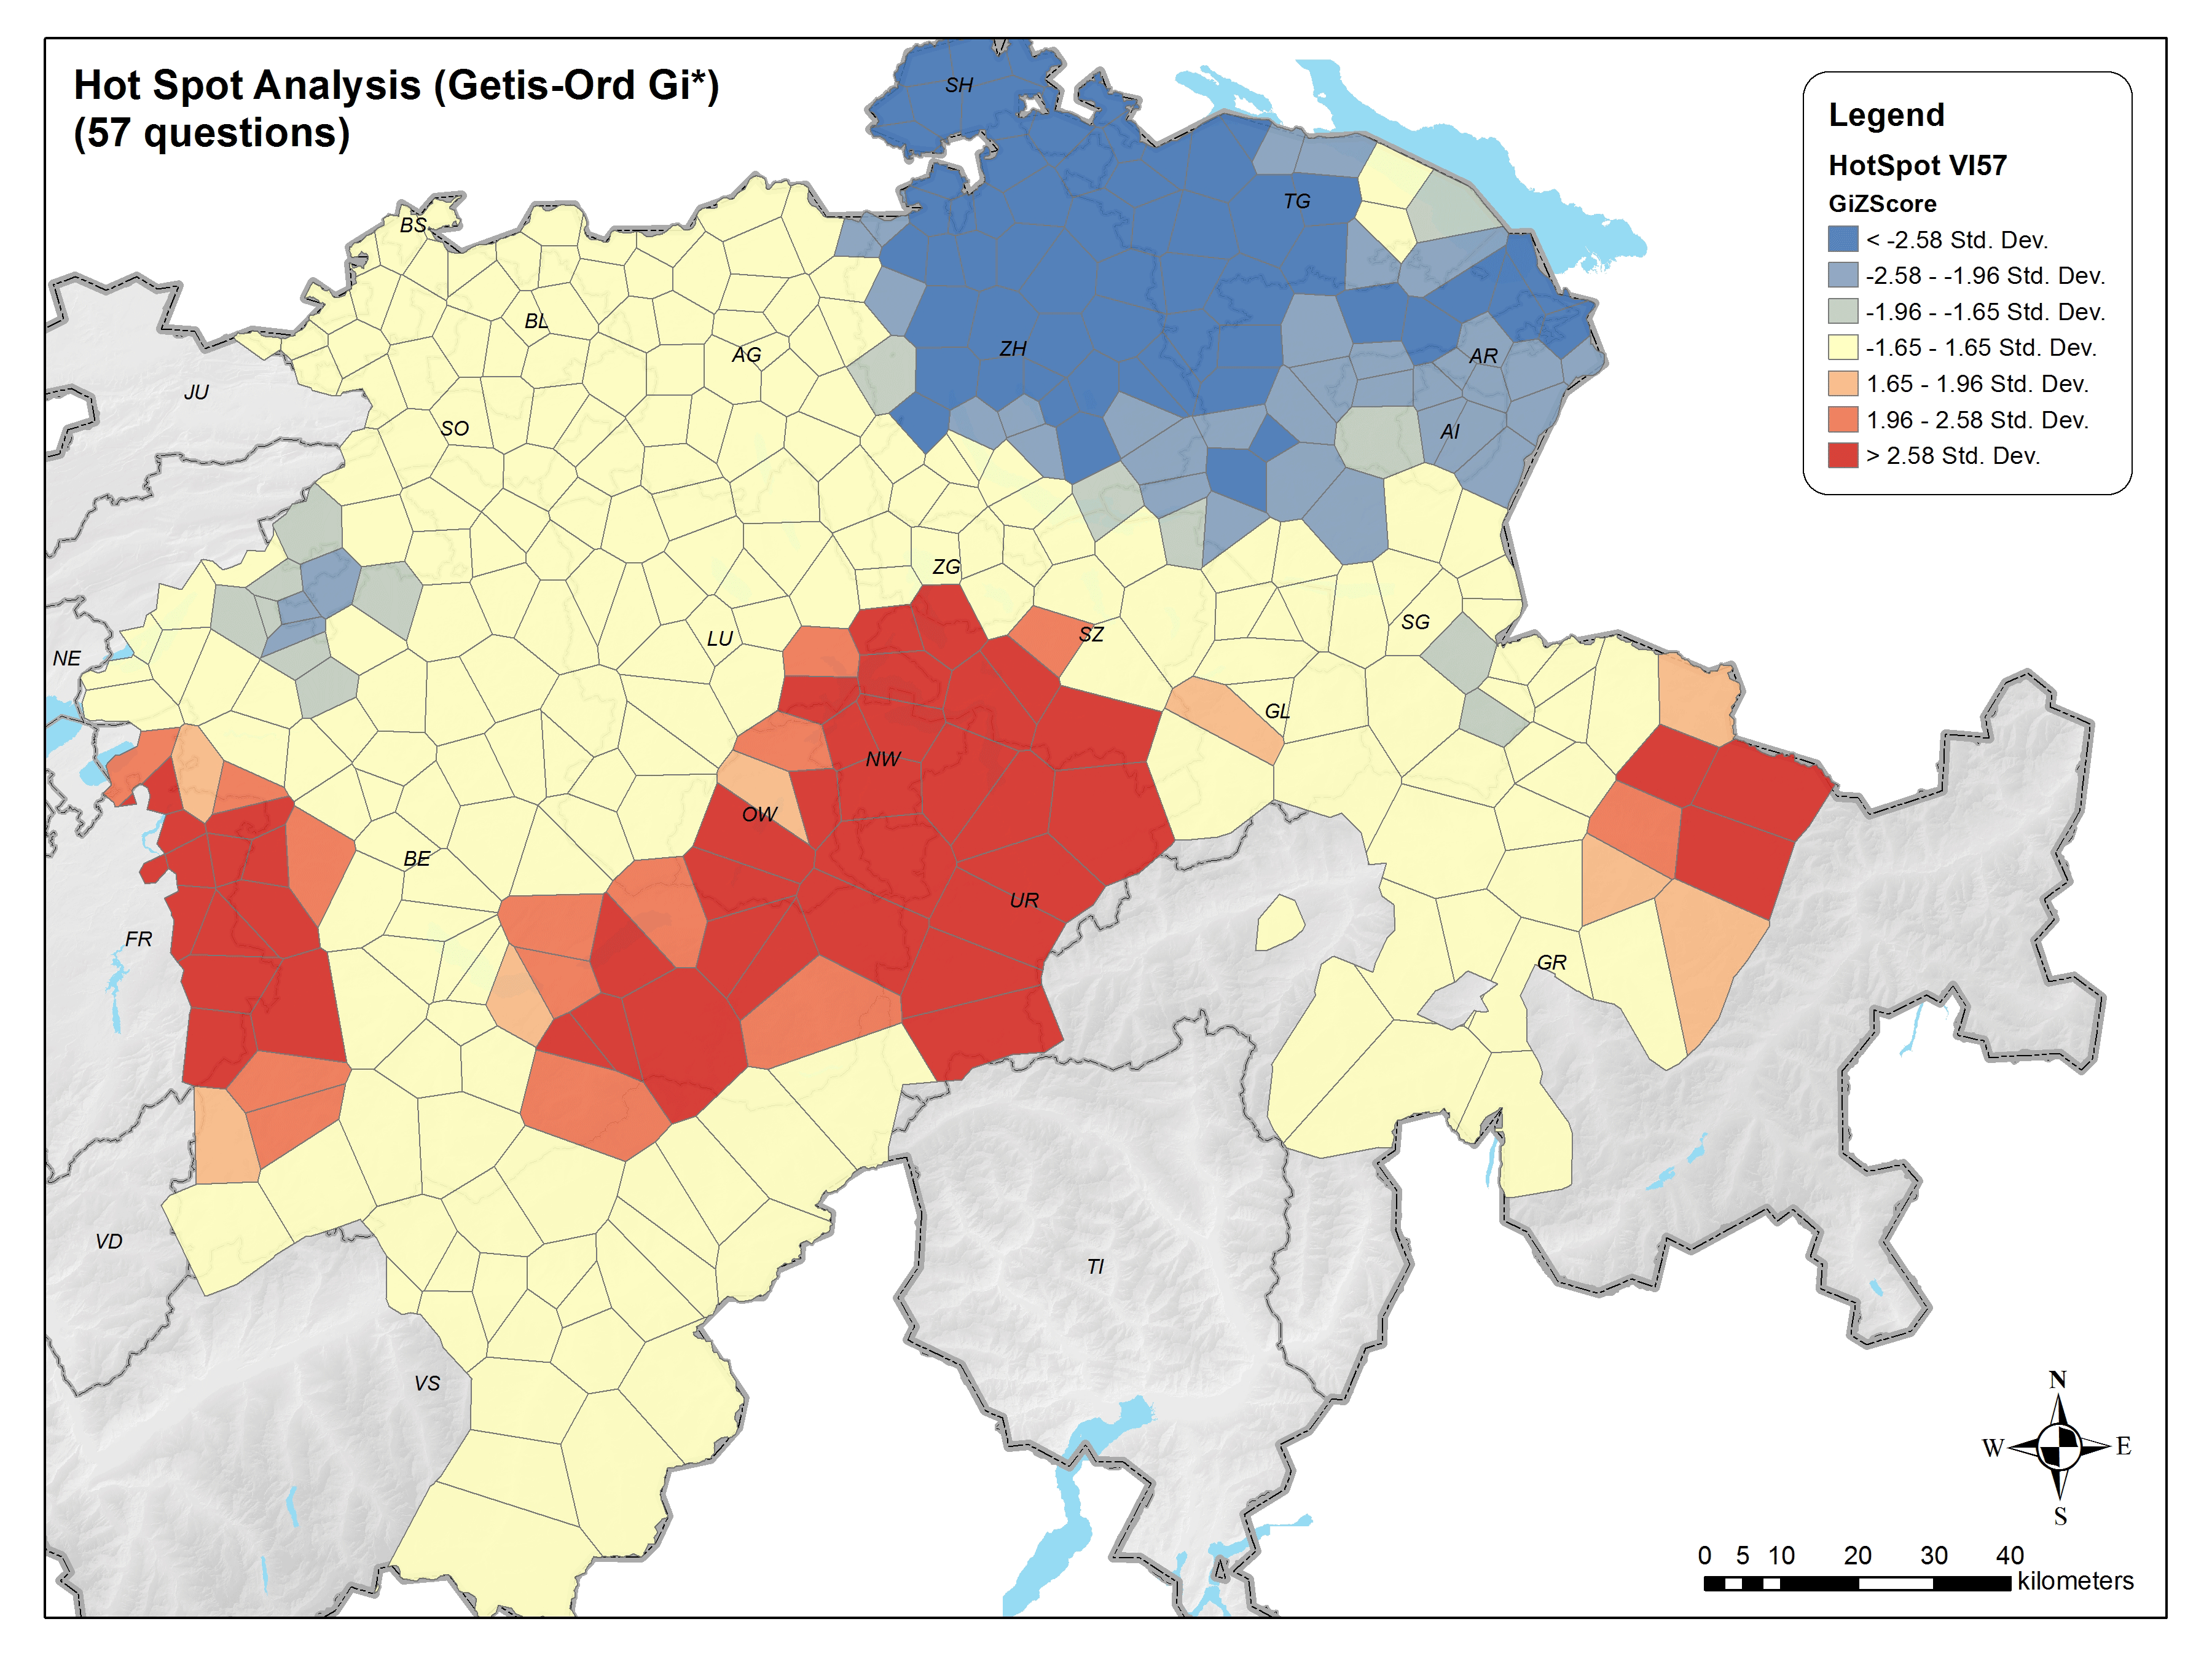
\includegraphics[width=\textwidth]{illustrations/stoeck_fig6}
\label{fig:6}
\caption{Hot Spot Analysis of the \emph{variation index} (Getis-Ord Gi* statistic; fixed distance band; Euclidean distance; distance threshold: 17.4km).}
\end{figure}

The map confirms the impression we gained from observing \figref{fig:5}: In the north-east we find a cluster of low \emph{VI} values or a cold spot (the blue areas), indicating little variation or high agreement between the informants regarding their answers. Furthermore, there is a smaller cluster of blue polygons in the west. On the other hand, there are three hot spots, i.e. clusters of high \emph{VI} values which indicate a lot of variation.\footnote{There is one more cold spot in the east. Since it only consists of two polygons, it will not be considered in the following.} Of course, one has to be careful interpreting the results, since changes in the analysis settings (e.g. autocorrelation method, distance method, etc.) can yield slightly different pictures. However, as modified analyses of the same data show,\footnote{ Besides the hot spot analysis, other techniques like cluster analysis using the local Moran’s I value or Kriging interpolation were applied to the data.} the general picture is very similar for each case: While agreement between the informants is rather high in the north-eastern region, especially central Switzerland but also the peripheral regions in the cantons of Fribourg and Grisons show a lot of variation. Before we engage in interpreting these findings, we will address the first question raised above, i.e. to what degree the choice of phenomena influences the results.

It is clear that the list of phenomena that were included in the SADS survey represents a selection of the many syntactic structures that could have been subject to linguistic research. Since the authors of the SADS put a lot of thought into the selection of relevant features \citep{bucheli_syntactic_2002}, we will not deal with this aspect of the question here. However, there is still the fact to consider that it was only possible to use 57 of the 118 SADS questions for our analysis of syntactic variation, a selection which could also have influenced the results. One way to deal with this problem is to build different subgroups of the dataset and see how much they correlate with the entire dataset. I therefore created six different subsets which are listed in the following:

\begin{itemize}
\item \emph{VI reduced}: The idea for this subset was to create a balanced dataset that does not contain any questions that display very similar geographic patterns. For this purpose, the pairwise correlations for all \emph{IDV}s were calculated. Finally, from the twelve pairs of questions with the highest correlations, one was omitted in each case, so that the subset consists of 45 instead of 57 SADS questions.
\item \emph{VI phenomena}: As previously mentioned, the 57 questions taken into account represent 26 different phenomena. In order to weight these phenomena equally, the arithmetic mean value was calculated for each of them. Therefore this subset consists of 26 phenomena.
\item \emph{VI M(ultiple) C(hoice)}: For this subset, all multiple choice questions (36 out of 57) were taken into account.
\item \emph{VI translation}: Analogously to \emph{VI MC}, all translation questions (21 out of 57) were taken into account.
\item \emph{VI random 1 \& 2}: Two subsets, each containing 30 randomly chosen questions, were created.
\end{itemize}

Each of these subgroups were correlated with VI all, i.e. the variation index that was calculated on the basis of all 57 questions. The results are shown in \tabref{tab:1}.

%%%
%%% alternatively: rotated text on top row
%%%
\begin{table}
\begin{tabular}{lllllll}
\lsptoprule
\begin{minipage}[t]{0.11\textwidth}\end{minipage}& 
\begin{minipage}[t]{0.11\textwidth}VI reduced\end{minipage} & 
\begin{minipage}[t]{0.11\textwidth}VI phenomena\end{minipage} & 
\begin{minipage}[t]{0.11\textwidth}VI MC\end{minipage} & 
\begin{minipage}[t]{0.11\textwidth}VI translation\end{minipage} & 
\begin{minipage}[t]{0.11\textwidth}VI random 1\end{minipage} & 
\begin{minipage}[t]{0.11\textwidth}VI random 2\end{minipage}\\
\midrule
VI all & .91 & .87 & .83 & .69 & .84 & .82\\
\lspbottomrule
\end{tabular}
\label{tab:1}
\caption{Correlations between VI for all 57 phenomena and VI s for different subsets (Pearson method, p-values for all correlations {\textless}.001)}
\end{table}

As the table shows, all correlations have high coefficients and are highly significant with p{\textless}.001. However, the correlations are not equally high: The subgroup \emph{VI reduced} shows the highest coefficient, followed by \emph{VI phenomena}, \emph{VI random 1}, \emph{VI MC}, \emph{VI random 2} and \emph{VI translation}. The different correlations are reflected in the respective geographic distributions, which show slight differences. Since the geographic patterns mainly differ with respect to the extensions of the hot and cold spots rather than their locations,\footnote{There are some minor exceptions which cannot be dealt with here.} we can state that the general variation pattern – a low variation index in the north-east vs. a high variation index in the southern areas – holds for all our subsets. For a more detailed account of the little differences it would be necessary to take a closer look at the individual questions from the different subgroups and perform more qualitative analyses with them. Moreover, it should be noted that the methods used to create the subsets differ clearly from each other: While \emph{VI reduced} and \emph{VI random 1 \& 2} were created for statistical reasons, the basis for building \emph{VI MC} and \emph{VI translation} was the elicitation method used in the questionnaire. \emph{VI phenomenon }was the only subset created on the basis of a linguistic classification. At this point it should be mentioned that it would be interesting to create further subgroups of that kind focusing on different grammatical domains such as NP, VP, word order etc. Of course, this would require more classification groundwork. The fact that different subsets of the data yield comparable results suggests that the variation index can be considered a quite stable measure for the syntactic variation in our research area.

\section{Discussion}

The starting point for this paper was the observation that dialectal variation can be analyzed not only on the geographical level, i.e. \emph{between} locations, but also \emph{within} locations, the latter being a merit of the SADS research design including multiple informants at each location. As the inspection of one phenomenon could show (and as many other studies of the SADS data have shown previously), variation occurs in many areas, but it does not appear to be chaotic. In order to get a grasp of the regional distribution of syntactic variation, the agreement rate between all informants at one place regarding the dominant variant was used to create a variation index. A quantification of this simple measure\footnote{ One could also think of more sophisticated measures like counting the actual number of occurring variants. However, these would have to be harmonized with the number of possible variants as well as with the number of informants in each case.} and its mapping to the SADS survey locations showed a characteristic geographic pattern with very little variation in the north-east and a lot of variation in central Switzerland and the peripheral regions in the cantons of Fribourg (\textsc{fr}) and Grisons (\textsc{gr}). A correlation with different subsets of the data showed that the general variation pattern still holds if a reduced version of the dataset is used.

However, so far we haven’t dealt with the question of how to interpret the findings. In many (socio)linguistic studies variation is regarded as an indicator for dynamism and linguistic change. In Swiss German dialectology the southern regions where most of our hot spots are located are generally considered rather conservative areas, whereas the north(east) is regarded as the part of Switzerland where the most innovations are found \citep{haas_deutschsprachige_2000}. So how do these results fit with our findings? If variation is considered an indicator of linguistic dynamics, the geographic pattern of syntactic variation seems to contradict the general findings regarding Swiss German dialects. As a first step toward an explanation we take a closer look at our three hot spots in the south and consider their different geographic contexts. With respect to the two areas in the eastern and western peripheries, we can state that they are both located in linguistic contact zones: the majority of the canton of Fribourg belongs to the French-speaking area, while in the canton of Grisons Romansh and Italian are spoken in addition to German.\footnote{ Though an influence of the neighboring Romance languages seems obvious, further analyses would be necessary to provide evidence.} Linguistically, the latter canton is especially interesting since for historical reasons its German-speaking inhabitants either speak a high Alemannic dialect which spread from the northern regions around the Rhine Valley and the Lake of Constance or a so-called “Walser German” (named after the canton of Wallis), a dialect which was brought by settlers during the Walser migrations that started in the Middle Ages.

Our largest hot spot is located in the center of Switzerland. In the linguistic literature two major dialectal contrasts are generally assumed to be important: one between North and South, the other between East and West \citep[61-67]{haas_deutschsprachige_2000}. Although these two divisions can be seen as generalizations of many linguistic differences with more or less similar geographic distributions, it is clear that central Switzerland is exposed to many different influences and is often seen as a dialectal transition zone.

If we take a closer look at our own data, we find that the areas with a high variation index – especially those located in the eastern and western peripheries – are those regions where in many cases very distinct variants can be found. Examples would be the missing article before personal names as in \emph{Ich habe Ø Fritz gesehen}\footnote{ Unlike standard German, the common variant used in most parts of German-speaking Switzerland is \textit{Ich habe den Fritz gesehen} with a definite article.} (‘I have seen Fritz’), or copredicative agreement as in \emph{Fischstäbchen gefroren-e anbraten} (fish fingers:\textsc{n.pl} frozen:\textsc{n.pl} fry; ‘to fry fish fingers frozen’; \citealt{berger_depictive_2005}). Interestingly, the latter variant is also found in the Wallis, often said to be the dialectally most conservative region in Switzerland. In contrast to the other southern areas, where this variant co-occurs with the other, more widespread ‘common’ form, in the Wallis it is the only variant.

Based on our findings, what conclusions can we draw regarding the dynamics of syntactic variation in German-speaking Switzerland? Our results suggest that variation and dynamism probably do not point to ‘modernism’, since they are found in the conservative, southern dialect areas. Rather, it seems that many of the forms that are dominant in the north-east are spreading toward the traditional areas which are dynamically being exposed to a lot of variation. Whether the inter-speaker syntactic variation is ‘stable’, i.e. distinct variants and more widespread variants continue to co-exist, or can be seen as an indicator for language change, is not clear at the present \citep{glaser_wandel_2014} and will be subject to future research. For this purpose it will be helpful to take a closer look at the sociolinguistic variables and see whether there are indicators for apparent-time change. Moreover, it will be interesting to compare the SADS findings with results from other dialect syntax projects which also have more than one informant per location (e.g. the \emph{Syntax hessischer Dialekte (SyHD)} ‘Syntax of Hessian dialects’; \citealt{fleischer_erhebung_2012}). 

\section*{Acknowledgements}
This paper is a revised and extended version of a talk I gave at the Methods in Dialectology XV conference in Groningen (NL), August 2014. I would like to thank Elvira Glaser, Péter Jeszenszky and Gabriela Bart for their helpful comments, as well as three anonymous referees. Moreover, I would like to thank Stephanie Schwenke for correcting my English. All shortcomings are my own responsibility.

\printbibliography[heading=subbibliography,notkeyword=this]
\end{document}